\documentclass[11pt,a4paper,]{article}
\usepackage{lmodern}

\usepackage{amssymb,amsmath}
\usepackage{ifxetex,ifluatex}
\usepackage{fixltx2e} % provides \textsubscript
\ifnum 0\ifxetex 1\fi\ifluatex 1\fi=0 % if pdftex
  \usepackage[T1]{fontenc}
  \usepackage[utf8]{inputenc}
\else % if luatex or xelatex
  \usepackage{unicode-math}
  \defaultfontfeatures{Ligatures=TeX,Scale=MatchLowercase}
\fi
% use upquote if available, for straight quotes in verbatim environments
\IfFileExists{upquote.sty}{\usepackage{upquote}}{}
% use microtype if available
\IfFileExists{microtype.sty}{%
\usepackage[]{microtype}
\UseMicrotypeSet[protrusion]{basicmath} % disable protrusion for tt fonts
}{}
\PassOptionsToPackage{hyphens}{url} % url is loaded by hyperref
\usepackage[unicode=true]{hyperref}
\hypersetup{
            pdftitle={Report on Happiness up to 2022},
            pdfborder={0 0 0},
            breaklinks=true}
\urlstyle{same}  % don't use monospace font for urls
\usepackage{geometry}
\geometry{a4paper, centering, text={16cm,25cm}}
\usepackage[style=apa,]{biblatex}
\addbibresource{references.bib}
\usepackage{longtable,booktabs}
% Fix footnotes in tables (requires footnote package)
\IfFileExists{footnote.sty}{\usepackage{footnote}\makesavenoteenv{long table}}{}
\usepackage{graphicx,grffile}
\makeatletter
\def\maxwidth{\ifdim\Gin@nat@width>\linewidth\linewidth\else\Gin@nat@width\fi}
\def\maxheight{\ifdim\Gin@nat@height>\textheight\textheight\else\Gin@nat@height\fi}
\makeatother
% Scale images if necessary, so that they will not overflow the page
% margins by default, and it is still possible to overwrite the defaults
% using explicit options in \includegraphics[width, height, ...]{}
\setkeys{Gin}{width=\maxwidth,height=\maxheight,keepaspectratio}
\IfFileExists{parskip.sty}{%
\usepackage{parskip}
}{% else
\setlength{\parindent}{0pt}
\setlength{\parskip}{6pt plus 2pt minus 1pt}
}
\setlength{\emergencystretch}{3em}  % prevent overfull lines
\providecommand{\tightlist}{%
  \setlength{\itemsep}{0pt}\setlength{\parskip}{0pt}}
\setcounter{secnumdepth}{5}

% set default figure placement to htbp
\makeatletter
\def\fps@figure{htbp}
\makeatother


\title{Report on Happiness up to 2022}

%% MONASH STUFF

%% CAPTIONS
\RequirePackage{caption}
\DeclareCaptionStyle{italic}[justification=centering]
 {labelfont={bf},textfont={it},labelsep=colon}
\captionsetup[figure]{style=italic,format=hang,singlelinecheck=true}
\captionsetup[table]{style=italic,format=hang,singlelinecheck=true}


%% FONT
\RequirePackage{bera}
\RequirePackage[charter,expert,sfscaled]{mathdesign}
\RequirePackage{fontawesome}

%% HEADERS AND FOOTERS
\RequirePackage{fancyhdr}
\pagestyle{fancy}
\rfoot{\Large\sffamily\raisebox{-0.1cm}{\textbf{\thepage}}}
\makeatletter
\lhead{\textsf{\expandafter{\@title}}}
\makeatother
\rhead{}
\cfoot{}
\setlength{\headheight}{15pt}
\renewcommand{\headrulewidth}{0.4pt}
\renewcommand{\footrulewidth}{0.4pt}
\fancypagestyle{plain}{%
\fancyhf{} % clear all header and footer fields
\fancyfoot[C]{\sffamily\thepage} % except the center
\renewcommand{\headrulewidth}{0pt}
\renewcommand{\footrulewidth}{0pt}}

%% MATHS
\RequirePackage{bm,amsmath}
\allowdisplaybreaks

%% GRAPHICS
\RequirePackage{graphicx}
\setcounter{topnumber}{2}
\setcounter{bottomnumber}{2}
\setcounter{totalnumber}{4}
\renewcommand{\topfraction}{0.85}
\renewcommand{\bottomfraction}{0.85}
\renewcommand{\textfraction}{0.15}
\renewcommand{\floatpagefraction}{0.8}


%\RequirePackage[section]{placeins}

%% SECTION TITLES


%% SECTION TITLES
\RequirePackage[compact,sf,bf]{titlesec}
\titleformat*{\section}{\Large\sf\bfseries\color[rgb]{0.7,0,0}}
\titleformat*{\subsection}{\large\sf\bfseries\color[rgb]{0.7,0,0}}
\titleformat*{\subsubsection}{\sf\bfseries\color[rgb]{0.7,0,0}}
\titlespacing{\section}{0pt}{2ex}{.5ex}
\titlespacing{\subsection}{0pt}{1.5ex}{0ex}
\titlespacing{\subsubsection}{0pt}{.5ex}{0ex}


%% TITLE PAGE
\def\Date{\number\day}
\def\Month{\ifcase\month\or
 January\or February\or March\or April\or May\or June\or
 July\or August\or September\or October\or November\or December\fi}
\def\Year{\number\year}

%% LINE AND PAGE BREAKING
\sloppy
\clubpenalty = 10000
\widowpenalty = 10000
\brokenpenalty = 10000
\RequirePackage{microtype}

%% PARAGRAPH BREAKS
\setlength{\parskip}{1.4ex}
\setlength{\parindent}{0em}

%% HYPERLINKS
\RequirePackage{xcolor} % Needed for links
\definecolor{darkblue}{rgb}{0,0,.6}
\RequirePackage{url}

\makeatletter
\@ifpackageloaded{hyperref}{}{\RequirePackage{hyperref}}
\makeatother
\hypersetup{
     citecolor=0 0 0,
     breaklinks=true,
     bookmarksopen=true,
     bookmarksnumbered=true,
     linkcolor=darkblue,
     urlcolor=blue,
     citecolor=darkblue,
     colorlinks=true}

\usepackage[showonlyrefs]{mathtools}
\usepackage[no-weekday]{eukdate}

%% BIBLIOGRAPHY

\makeatletter
\@ifpackageloaded{biblatex}{}{\usepackage[style=authoryear-comp, backend=biber, natbib=true]{biblatex}}
\makeatother
\ExecuteBibliographyOptions{bibencoding=utf8,minnames=1,maxnames=3, maxbibnames=99,dashed=false,terseinits=true,giveninits=true,uniquename=false,uniquelist=false,doi=false, isbn=false,url=true,sortcites=false}

\DeclareFieldFormat{url}{\texttt{\url{#1}}}
\DeclareFieldFormat[article]{pages}{#1}
\DeclareFieldFormat[inproceedings]{pages}{\lowercase{pp.}#1}
\DeclareFieldFormat[incollection]{pages}{\lowercase{pp.}#1}
\DeclareFieldFormat[article]{volume}{\mkbibbold{#1}}
\DeclareFieldFormat[article]{number}{\mkbibparens{#1}}
\DeclareFieldFormat[article]{title}{\MakeCapital{#1}}
\DeclareFieldFormat[article]{url}{}
%\DeclareFieldFormat[book]{url}{}
%\DeclareFieldFormat[inbook]{url}{}
%\DeclareFieldFormat[incollection]{url}{}
%\DeclareFieldFormat[inproceedings]{url}{}
\DeclareFieldFormat[inproceedings]{title}{#1}
\DeclareFieldFormat{shorthandwidth}{#1}
%\DeclareFieldFormat{extrayear}{}
% No dot before number of articles
\usepackage{xpatch}
\xpatchbibmacro{volume+number+eid}{\setunit*{\adddot}}{}{}{}
% Remove In: for an article.
\renewbibmacro{in:}{%
  \ifentrytype{article}{}{%
  \printtext{\bibstring{in}\intitlepunct}}}

\AtEveryBibitem{\clearfield{month}}
\AtEveryCitekey{\clearfield{month}}

\makeatletter
\DeclareDelimFormat[cbx@textcite]{nameyeardelim}{\addspace}
\makeatother

\author{\sf{\Large\textbf{(Elvis) Zhixiang Yang}\\\large EBS Honours Student\\[0.5cm]}{\Large\textbf{Yiqi Wang}\\\large Master of BA Student\\[0.5cm]}{\Large\textbf{Xintong You}\\\large Master of BA Student\\[0.5cm]}}

\date{\sf\Date~\Month~\Year}
\makeatletter
\lfoot{\sf Yang, Wang, You: \@date}
\makeatother


%%%% PAGE STYLE FOR FRONT PAGE OF REPORTS

\makeatletter
\def\organization#1{\gdef\@organization{#1}}
\def\telephone#1{\gdef\@telephone{#1}}
\def\email#1{\gdef\@email{#1}}
\makeatother
  \organization{Group 07 ETC5513}

  \def\name{Department of\newline Econometrics \&\newline Business Statistics}

  \telephone{(03) 9905 2478}

  \email{BusEco-Econometrics@monash.edu}

\def\webaddress{\url{http://buseco.monash.edu/ebs/consulting/}}
\def\abn{12 377 614 012}
\def\extraspace{\vspace*{1.6cm}}
\makeatletter
\def\contactdetails{\faicon{phone} & \@telephone \\
                    \faicon{envelope} & \@email}
\makeatother

\usepackage[absolute,overlay]{textpos}
\setlength{\TPHorizModule}{1cm}
\setlength{\TPVertModule}{1cm}

%%%% FRONT PAGE OF REPORTS

\def\reporttype{Report for}

\long\def\front#1#2#3{
\newpage
\begin{textblock}{7}(12.7,28.2)\hfill

\includegraphics[height=0.6cm]{AACSB}~~~

\includegraphics[height=0.6cm]{EQUIS}~~~

\includegraphics[height=0.6cm]{AMBA}
\end{textblock}
\begin{singlespacing}
\thispagestyle{empty}
\vspace*{-1.4cm}
\hspace*{-1.4cm}
\hbox to 16cm{
  \hbox to 6.5cm{\vbox to 14cm{\vbox to 25cm{
    
\includegraphics[width=6cm]{monash2}
    \vfill
    
\includegraphics[width=3.5cm]{MBSportrait}
    \vspace{0.4cm}
    \par
    \parbox{6.3cm}{\raggedright
      \sf\color[rgb]{0.00,0.00,0.70}
      {\large\textbf{\name}}\par
      \vspace{.7cm}
      \tabcolsep=0.12cm\sf\small
      \begin{tabular}{@{}ll@{}}\contactdetails
      \end{tabular}
      \vspace*{0.3cm}\par
      ABN: \abn\par
    }
  }\vss}\hss}
  \hspace*{0.2cm}
  \hbox to 1cm{\vbox to 14cm{\rule{1pt}{26.8cm}\vss}\hss\hfill}
  \hbox to 10cm{\vbox to 14cm{\vbox to 25cm{
      \vspace*{3cm}\sf\raggedright
      \parbox{11cm}{\sf\raggedright\baselineskip=1.2cm
         \fontsize{24.88}{30}\color[rgb]{0.70,0.00,0.00}\sf\textbf{#1}}
      \par
      \vfill
      \large
      \vbox{\parskip=0.8cm #2}\par
      \vspace*{2cm}\par
      \reporttype\\[0.3cm]
      \hbox{#3}%\\[2cm]\
      \vspace*{1cm}
      {\large\sf\textbf{\Date~\Month~\Year}}
   }\vss}
  }}
\end{singlespacing}
\newpage
}

\makeatletter
\def\titlepage{\front{\expandafter{\@title}}{\@author}{\@organization}}
\makeatother

\usepackage{setspace}
\setstretch{1.5}

%% Any special functions or other packages can be loaded here.
\usepackage{booktabs}
\usepackage{longtable}
\usepackage{array}
\usepackage{multirow}
\usepackage{wrapfig}
\usepackage{float}
\usepackage{colortbl}
\usepackage{pdflscape}
\usepackage{tabu}
\usepackage{threeparttable}
\usepackage{threeparttablex}
\usepackage[normalem]{ulem}
\usepackage{makecell}
\usepackage{xcolor}


\begin{document}
\titlepage

{
\setcounter{tocdepth}{2}
\tableofcontents
}
\clearpage

\hypertarget{introduction}{%
\section{Introduction}\label{introduction}}

\textcite{rojas2010} stated that there are many factors may contributing happiness.They also mentioned that conceptions of happiness differ not only across people, but also across the culture, region etc. There are so many of factors that can influence the happiness of people. If we want to improve the happiness of people, we cannot stimulate all the variables that are relevant. Thus, an analysis on the world happiness report will help to figure the common key variable that influence the happiness of human beings and the situation of happiness around the world. Then, we can try to give a better scope of happiness at a worldwide level, especially after the pandemic.

This report will analyse the happiness score of each country and different regions across the world to utilize the happiness at a world wide level. In order to capture the changes, there are various factors that relevant to the happiness score will be used to explain the variation of happiness score in different countries.

Apart from this, \textcite{helliwell2021world} stated that the global pandemic has significantly influenced the happiness of people in different regions. In considering of the pandemic, we also analyse the influence of COVID-19 to the rank of the happiness score in top countries and the variable relationships after the pandemic year 2020.

In the modelling part, we will provide an detailed analysis of the model fits in various models. In this part,we will illustrate the most important variables in explaining the happiness score. Furthermore, we will also add two new variables together with the important variables to build up a multivariate linear model based on the 4 variables between 2016 to 2020 and explore their marginal effects on the happiness scores.

However, due to the number of countries observed in different years are not consistent and variables are varies after year 2020, which might generate errors. Also, the new data are limited between 2016 to 2020, which can lead to sample selection bias. We will critically explain these issues in residual diagnostic part at the end of the modelling part.

\hypertarget{data}{%
\section{Data}\label{data}}

\hypertarget{description}{%
\subsection{Description}\label{description}}

Our data comes from Kaggle, which is a report of the World Happiness. In the eight datasets, the variables explaining the happiness score including Economy(measured in GDP per capita), Health status, Freedom, Generosity are consistent each year. Nevertheless, after year 2020, few new variables have been added and there are few changes with the existing variables. The happiness score is ranked from the highest to the lowest one and gained via an anonymous worldwide survey across different countries around the world.

Apart from our existing data, we will also join two new datasets in the modelling part gained from the World Bank Data due to the potential issues in our existing dataset. More information will be discussed in the multivariate linear model part.

\hypertarget{pre-processing.}{%
\subsection{Pre-processing.}\label{pre-processing.}}

The data gained from Kaggle is not clean. In this report, we tried to combine all the historical data with common factors, which are Economy, Health, Freedom, Generosity each year and drop the NA values. However, for specific yearly analysis after 2020, we decide to keep all the new variable in explaining the happiness score.

In addition, two variable related to Consumer Price Index and Populations will be joined across different countries in each year when we trying to build up our multivariate linear model.

\hypertarget{exploratory-data-analysis-world-happiness-from-2015-to-2022}{%
\section{Exploratory Data Analysis (World Happiness from 2015 to 2022)}\label{exploratory-data-analysis-world-happiness-from-2015-to-2022}}

In this part, we will investigate the trends of happiness score represented by region between 2015 and 2022. After this, we will analyse the impacts of annual health and economic status on happiness score.

Combined with my research questions, I consolidate all the datasets for each year betweeen 2015 to 2022 into a new dataset, and then tease out the variables to use, which are year, region, happiness score, economy, and health.

\hypertarget{the-development-of-the-world-happiness}{%
\subsection{The development of the World Happiness}\label{the-development-of-the-world-happiness}}

\textcite{helliwell2012state} stated that with the continuous progress of human society, the happiness index has become an important indicator for measuring the living standards across regions. Meanwhile, people have also realized the importance to apply the happiness index in macroeconomic analysis. In the real world, the happiness index is related to many factors, it will also affect nearly all aspects of human activities. Thus, we will start with two research questions to explore the happiness index of the world.

\hypertarget{research-questions}{%
\subsection{Research questions}\label{research-questions}}

\begin{itemize}
\item
  How will happiness trends change between 2015 to 2022 in different regions?
\item
  What is the relationship impacts of economic situation and health status to the happiness score?
\end{itemize}

\hypertarget{the-trends-in-happiness-2015-2022}{%
\subsection{The trends in happiness 2015-2022}\label{the-trends-in-happiness-2015-2022}}

\begin{figure}
\centering
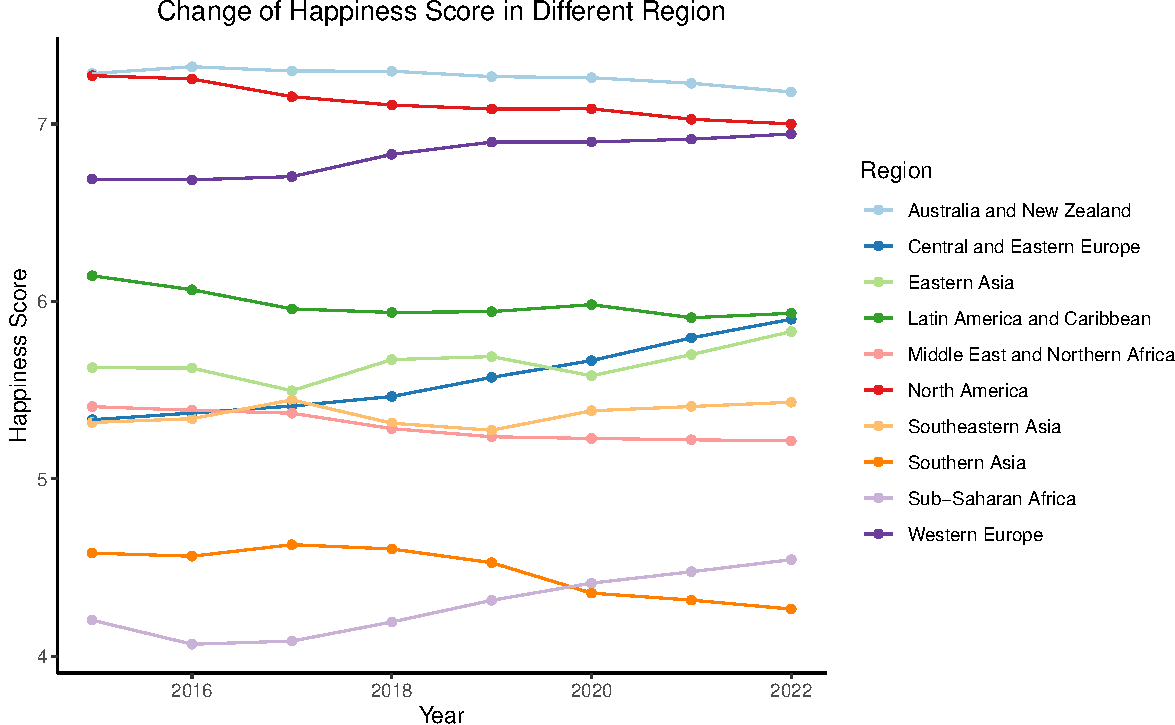
\includegraphics{Assignment4_files/figure-latex/trends-1.pdf}
\caption{\label{fig:trends}Change of Happiness Score in Different Region}
\end{figure}

From the Figure \ref{fig:trends}, we can see that the trend in all regions can be divided into three different levels of happiness score.

We can see from the plot that South Asia and Sub-Saharan Africa remained at low level for the past few years. While Southern Asia countries started declining in 2017, Sub-Saharan Africa's happiness began to increase year by year after reaching the trough in 2016. In addition, the declining trend of happiness for people in Southeastern Asia may due to the population booming in these years.

The three regions with the highest overall happiness are: Australia and New Zealand, North America, and Western Europe. We can see people living in these developed area feels happier than others, which may be due to the good social welfares, less stress and better working environment. Nevertheless, an interesting point to notice is that even there are many modern countries in Eastern Asia, people didn't really feel happy in the past few years. This may due to the living condition and working stresses are high from these Eastern Asian countries.

Then, we can see the remaining regions are all centered in middle level. Among these regions, Central and Eastern Europe is the only region have an obvious increasing trend over the years, while the rest of the region is in a state of slightly fluctuating but generally stable trends.

Overall, we conclude that for those regions with relatively better economic situation and social welfare would generally lead to a higher happiness scores with less fluctuations than those regions with poor economic situation.

\hypertarget{the-relationship-between-economic-situation-and-health-status-with-the-happiness-in-2015-2022}{%
\subsection{The relationship between economic situation and health status with the happiness in 2015-2022}\label{the-relationship-between-economic-situation-and-health-status-with-the-happiness-in-2015-2022}}

People's understanding of happiness is inseparable from their own living conditions. In this section, we will also explore the relationship between happiness and economic and health status.

From the figure \ref{fig:VS}, we can find that there is a positive correlation between economic status, health status and happiness score from 2015 to 2022, which is make sense that a better the economic status and health status will make people happier.

There is an overall trend from 2015 to 2022 that the correlation of health and happiness is increasing over the years. Nevertheless, the correlation of economic situation is decreasing. This may due to the situation that people have better economic situation nowadays and they pay more attention on their health status.

From 2017 to 2018, the average influences of economic on happiness score increased slightly, while the influence of health on happiness score decreased slightly during this period.

From 2019 to 2022, the influence of the economic status on the happiness score is getting lower while the influence of the health on the happiness score has increased significantly especially after 2020, which maybe due to the pandemic that people care more about their health status.

\begin{figure}
\centering
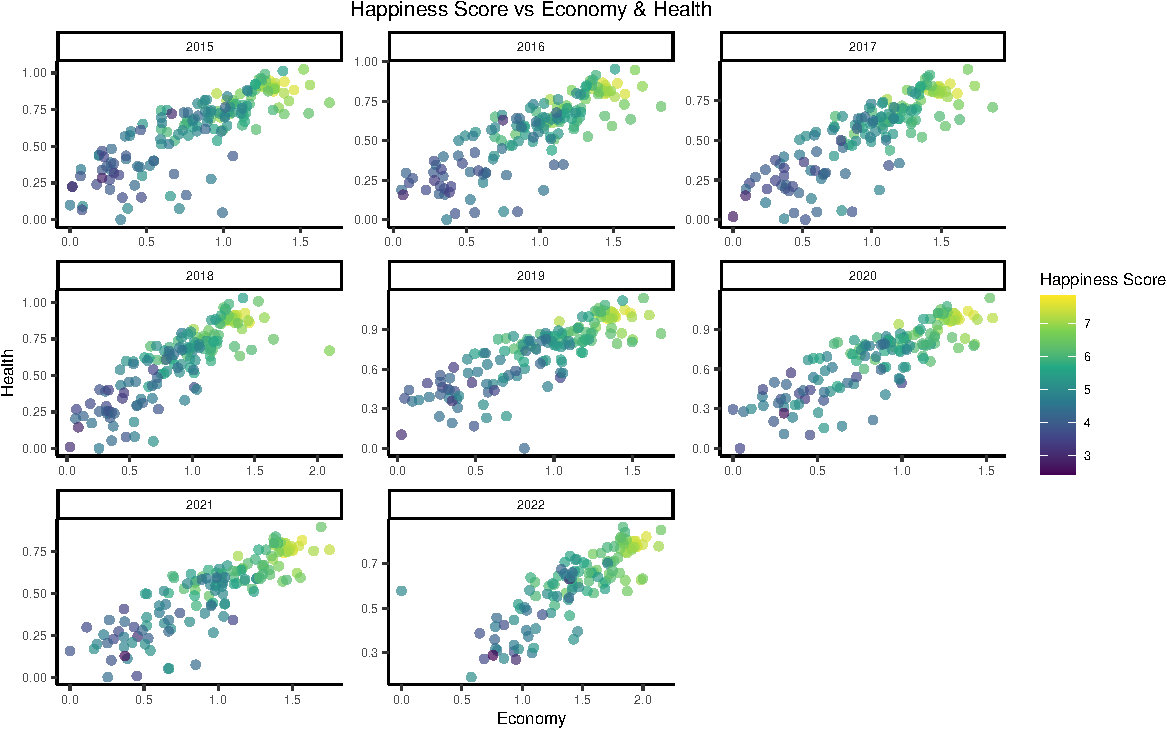
\includegraphics{Assignment4_files/figure-latex/VS-1.pdf}
\caption{\label{fig:VS}Happiness Score vs Economy \& Health}
\end{figure}

\newpage

\begin{table}
\centering
\begin{tabular}{|c|c|c|c|}
\hline
\textbf{Year} & \textbf{Intercept} & \textbf{Economy} & \textbf{Health} \\
\hline
2015          & 3.250              & 1.616            & 1.203           \\
2016          & 2.980              & 1.516            & 1.662           \\
2017          & 2.968              & 1.504            & 1.632           \\
2018          & 3.085              & 1.511            & 1.565           \\
2019          & 2.892              & 1.359            & 1.775           \\
2020          & 3.117              & 1.305            & 1.791           \\
2021          & 3.298              & 1.316            & 1.854           \\
2022          & 2.370              & 1.406            & 2.085           \\
\hline
\end{tabular}
\caption{A linear relationship between economic status and health status with happiness index each year}
\label{tab:table}
\end{table}

We also conducted an simple regression analysis. From the Table \ref{tab:table}, we can see the impact of economic situation on the slope decreased very slowly from 1.616 to 1.406 over the years. On the contrary, the influence of health on happiness score changed a lot with the slope increased from 1.2 to 2.08. Through this simple linear regression analysis, we can also see that people gradually focus on their health status nowadays.

\hypertarget{exploratory-data-analysis-pandemic-influences}{%
\section{Exploratory data analysis (Pandemic Influences)}\label{exploratory-data-analysis-pandemic-influences}}

\hypertarget{introduction-1}{%
\subsection{Introduction}\label{introduction-1}}

According to \textcite{helliwell2021world}, economic situation, people's health and freedom have been severely affected across different countries since the outbreak of COVID-19 in 2020, which will directly impact the world.

In the following research, the top 10 happiest countries in the world and their regions will be explored. Then, factors associated with the happiness score will be explored by analyzing the relation between happiness score and six selected indicators in 2021.

\hypertarget{what-are-the-countries-which-ranks-top-10-in-happiness-score-since-the-covid-19-outbreak}{%
\subsection{What are the countries which ranks top 10 in happiness score since the COVID-19 outbreak?}\label{what-are-the-countries-which-ranks-top-10-in-happiness-score-since-the-covid-19-outbreak}}

\begin{figure}
\centering
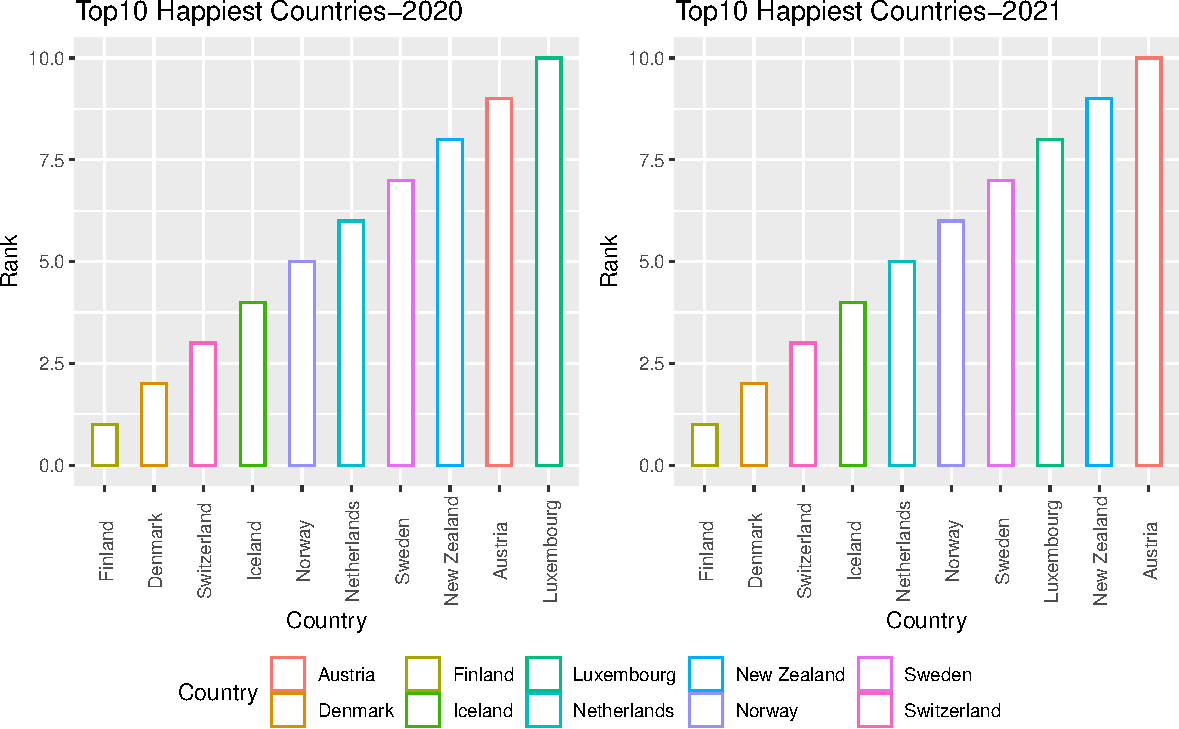
\includegraphics{Assignment4_files/figure-latex/top10-1.pdf}
\caption{\label{fig:top10}The top 10 countries in happiness score since COVID-19}
\end{figure}

In the Figure \ref{fig:top10}, the top 10 countries in the World Happiness have not changed since 2020 despite the impact of COVID-19, while their ranks have changed slightly.

In addition, Finland has been the happiest country for two consecutive years in 2020 and 2021. We believe this is mainly due to the fact that Finland has a well structured social welfare and health care system \autocite{lappi2006finland}.

\hypertarget{the-distribution-of-the-top-10-countries-on-the-world-map-in-2021}{%
\subsection{The distribution of the top 10 countries on the world map in 2021}\label{the-distribution-of-the-top-10-countries-on-the-world-map-in-2021}}

\begin{verbatim}
## 10 codes from your data successfully matched countries in the map
## 0 codes from your data failed to match with a country code in the map
## 233 codes from the map weren't represented in your data
\end{verbatim}

\begin{figure}
\centering
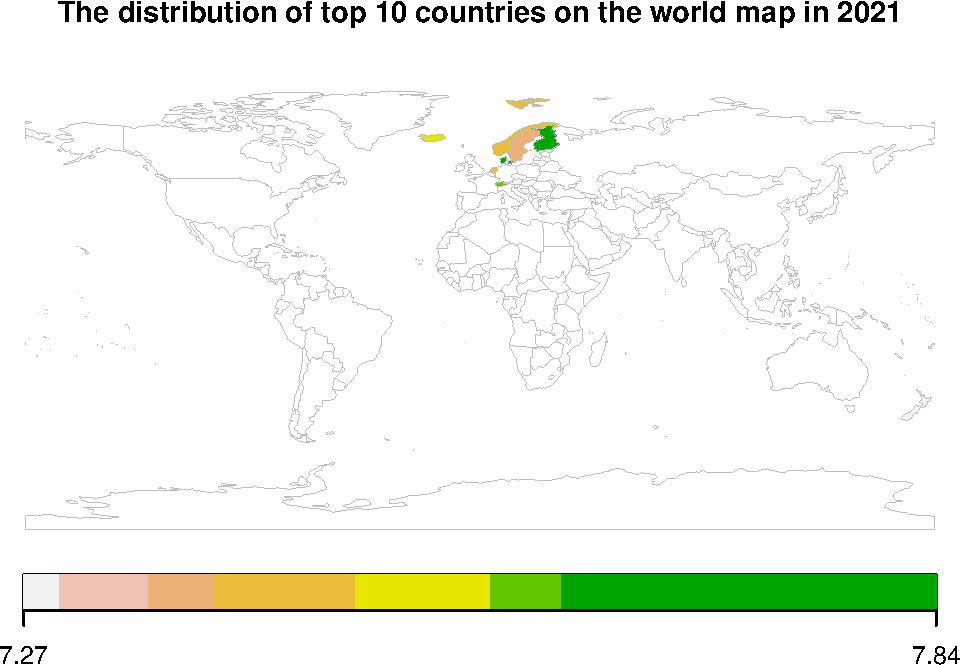
\includegraphics{Assignment4_files/figure-latex/top10map-1.pdf}
\caption{\label{fig:top10map}The distribution of top 10 countries on the world map in 2021}
\end{figure}

According to the Figure \ref{fig:top10map}, these countries are mainly northern and western European countries, obviously, they are all developed countries which have a technologically advanced infrastructure, and their economy is highly developed.

So besides high economy, what other indicators can affect happiness score?

\hypertarget{relation-between-happiness-score-and-other-indicators-in-2021}{%
\subsection{Relation between Happiness score and other indicators in 2021}\label{relation-between-happiness-score-and-other-indicators-in-2021}}

\begin{figure}
\centering
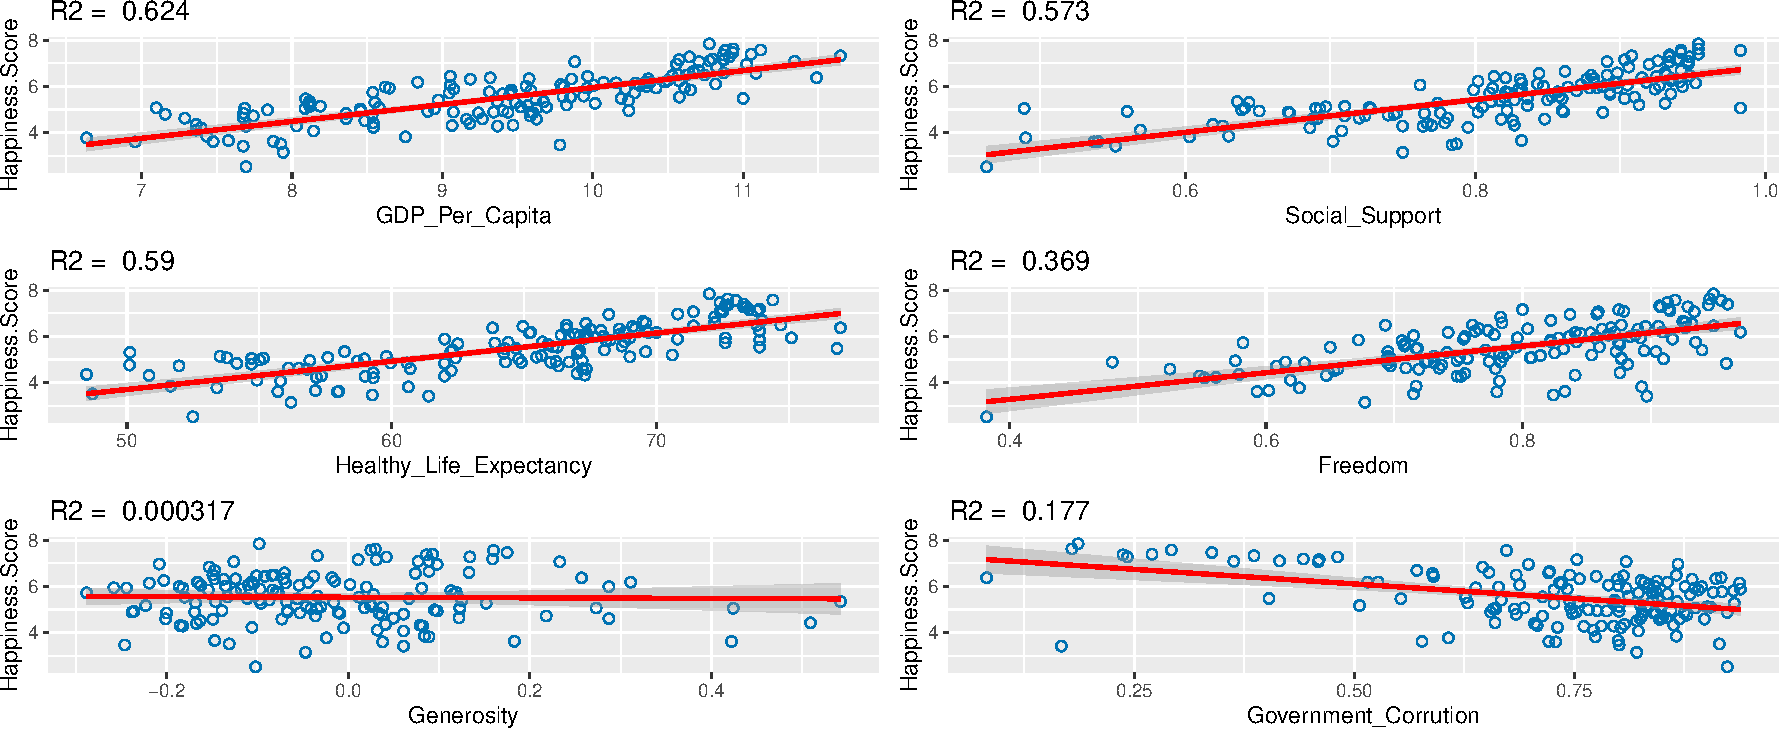
\includegraphics{Assignment4_files/figure-latex/relation-1.pdf}
\caption{\label{fig:relation}Relation between Happiness score and 6 indicators in 2021}
\end{figure}

The 6 linear graphs Figure \ref{fig:relation} demonstrate the relation between the happiness and 6 attributes of the countries in the world in 2021. R-squared(R2) represents the proportion of the variance for happiness that's explained by an independent variable in the regression model. For example, in the graph on the upper left, its R-squared is 0.624, indicating that there are 62.4\% of countries' GDP can explain their happiness.

Therefore, social support and health life expectancy explain happiness in a relatively high proportion which is 57.3\% and 59\% respectively. While freedom, generosity and trust in government corruption are not good explanations for happiness score.

\hypertarget{conclusion}{%
\section{Conclusion}\label{conclusion}}

In conclusion, the world's top 10 happiest countries are mainly concentrated in Northern and Western Europe in 2020 and 2021, which have high economic level and GDP. From the data of the world, the variables highly related to happiness are \textbf{GDP, social support and health life expectancy}.

\hypertarget{conclusions}{%
\subsection{Conclusions}\label{conclusions}}

Through our exploration of two research questions, we found that in economically developed countries, people's happiness is also higher, while people's happiness in economically backward areas will also be lower; and with the continuous progress of society, people's happiness comes from the impact of health, especially in the stage of covid-19. In general, some European countries and some developed countries have better welfare and medical security for their own developed economies, and people's happiness is also very high. On the contrary, in some economically poor areas, their welfare security is also poor, which also makes the happiness of the people not high.

\printbibliography

\end{document}
